\section{Introduction}

%Introductory section which may include references in parentheses
%\citep{R}, or cite a reference such as \citet{R} in the text.

%\subsubsection*{Significance.}
The segmentation of a network into communities such that individuals in the same community share similar features, whilst individuals across communities are dissimilar is a technique known as clustering, and is a principal task in the analysis of networks. This can be achieved by various algorithms that differ significantly in their understanding of what constitutes a community (or cluster) and in the way to find them. 
Once a clustering algorithm is selected, the user is faced with the problem of 
 determining how meaningful the clusters obtained are. Here is where \CRANpkg{clustAnalytics} comes into play. 
 
 \CRANpkg{clustAnalytics} contains a suite of 
novel methods to validate the  partitions  of  networks obtained by any given clustering algorithm. 
In particular, its clustering validation methods focus on two of the most important aspects of cluster assessment: the {\em significance} and the {\em stability} of the resulting clusters.
Clusters produced by a clustering algorithm are considered to be {\em significant} if there are  strong connections within each cluster, and weaker connections (or fewer edges) between different clusters. 
%%%
On the other hand, {\em stability} measures how much a clustering remains unchanged under small perturbations of the network. In the case of weighted networks, these could include the addition and removal of vertices, as well as the perturbation of edge weights. 

\CRANpkg{clustAnalytics} handles weighted networks (that is, those in which the connections between nodes have an assigned numerical value representing some property of the data), as well as unweighted, and contains several other functionalities for producing different statistics on a network, and measures of similarity of partitions produced by two different clustering algorithms, most notably an enhanced version of the Reduced Mutual Information (RMI) of \cite{corrected_MI_Newman2020}.
In the following sections we introduce some examples of usage and highlight the principal tasks resolved by \CRANpkg{clustAnalytics}.

\section{Background concepts}

Community detection on networks, which are represented by graphs, is a very active topic of research with many applications. The \CRANpkg{igraph} \citep{igraph} package contains a collection of the most popular algorithms for this task, such as the Louvain \citep{fastunfolding}, walktrap \citep{walktrap} and label propagation \cite{label_propagation} algorithms.


Evaluating the significance of the community structure of a network is no simple task, because there is not an authoritative definition of what a significant community is. However, there is some agreement in the literature (see the survey by \cite{Fortunato2010}) in that communities should have high internal connectivity (presence of edges connecting nodes in the community) while being well separated from each other. These notion can be quantified and formalized by applying several community {\em scoring functions} (also known as quality functions  in \citep{Fortunato2010}), that gauge either the intra-cluster or inter-cluster density. \CRANpkg{clustAnalytics} implements the most relevant, or representative, community scoring functions following the 
taxonomy of these quality measures done by \cite{groundtruth} and the further discussion on how to adapt them to weighted networks in \citep{arratia2021clustering}.

However, to evaluate the significance of clusters on a given network, one needs reference values of the scoring functions to determine whether they are actually higher than those of a comparable network with no community structure. For this, we use a method described in \citep{arratia2021clustering} that rewires edges (or transfers some of their weight, in the case of weighted networks) while keeping the degree distribution constant. Then, it can be determined that the partition of a network contains significant clusters if it obtains sufficiently
better scores than those for a comparable network with uniformly distributed edges. 


%\subsubsection*{Stability.} 
On the other hand, stability measures how much the partition of a network into communities remains unchanged under small perturbations. In the case of weighted networks, these could include the addition and removal of vertices, as well as the perturbation of edge weights. This is consistent with the idea that meaningful clusters should capture an inherent structure in the data and not be overly sensitive to small or local variations, or the particularities of the clustering algorithm. To measure the variation that such perturbations present in the clusters, there are multiple similarity metrics available. We have selected for inclusion the Variation of Information \citep{varinformation}, the Reduced Mutual Information \citep{corrected_MI_Newman2020}, and the Rand Index (both in its original and adjusted forms) \citep{Hubert1985}. The first two are based on information theory, while the second one counts agreements and disagreements in the membership of pairs of elements. Then, it is possible to evaluate the network using resampling methods such as nonparametric bootstrap, as described for clustering on Euclidean data by \cite{Hennig2007}, and later for networks by \cite{arratia2021clustering}, and quantify the deviations from the initial partition with the similarity measures.



\section{The \textit{clustAnalytics} package} 

The  \textit{clustAnalytics} package (version 0.5.4) contains  23 functions for assessing  clustering significance and stability, and other useful utilites. These are listed in Table \ref{functions_table} grouped by category. It also contains some  auxiliary functions to support package management and provide useful baseline graphs with communities. Check these in the reference manual. In what follows we detail the usage of the main functions.


% Please add the following required packages to your document preamble:
% \usepackage{multirow}
\begin{table}[]
\small
\begin{tabular}{|cl|l|}
\hline
\multicolumn{1}{|c|}{\multirow{4}{*}{significance}} & \multirow{2}{*}{\begin{tabular}[c]{@{}l@{}}scoring\\ functions\end{tabular}} & \texttt{scoring\_functions(g, com, type , weighted, w\_max)}                                                                                                                                                                                                                                                                                                      \\ \cline{3-3} 
\multicolumn{1}{|c|}{}                              &                                                                              & \begin{tabular}[c]{@{}l@{}}\texttt{average\_degree, average\_odf, conductance, coverage,}\\ 
\texttt{cut\_ratio, density\_ratio, edges\_inside, expansion, FOMD,}\\ 
\texttt{internal\_density, max\_odf, normalized\_cut,}\\ \texttt{weighted\_clustering\_coefficient, weighted\_transitivity} \end{tabular}                                                                                  \\ \cline{2-3} 
\multicolumn{1}{|c|}{}                              & \begin{tabular}[c]{@{}l@{}}graph \\ rewiring\end{tabular}                    & \begin{tabular}[c]{@{}l@{}} \texttt{rewireCpp(g, Q=100, weight\_sel="const\_var", lower\_bound=0,}\\ \texttt{\ \ \ \ \ \ \ \ \ \ upper\_bound=NULL)} \end{tabular}                   \\ \cline{2-3} 
\multicolumn{1}{|c|}{}  & evaluation                                                                   & \begin{tabular}[c]{@{}l@{}}\texttt{evaluate\_significance(g, alg\_list, gt\_clustering, w\_max)}\\ 
\texttt{evaluate\_significance\_r(g, alg\_list, gt\_clustering,}\\ 
\texttt{\ \ \ \ \ \ \ \ \ \ \ \ \ \ \ \ \ \ \ \ \ \ \ \ Q=100, lower\_bound=0, w\_max=NULL,}\\
\texttt{\ \ \ \ \ \ \ \ \ \ \ \ \ \ \ \ \ \ \ \ \ \ \ \ table\_style = "default")}\end{tabular}
\\ \hline
\multicolumn{2}{|l|}{stability}                                                                                                    & \begin{tabular}[c]{@{}l@{}}\texttt{boot\_alg\_list(g, alg\_list, R=999, return\_data=FALSE, }\\
\texttt{\ \ \ \ \ \ \ \ \ \ \ \ \ \ type="global")}\\
\texttt{reduced\_mutual\_information(c1, c2, base=2, normalized=FALSE, }\\                    \texttt{\ \ \ \ \ \ \ \ \ \ \ \ \ \ \ \ \ \ \ \ \ \ \ \ \ \ \ method="approximation2")}\end{tabular}                                                                                             \\ \hline
\multicolumn{2}{|l|}{other functions}                                                                                              & \begin{tabular}[c]{@{}l@{}}
\texttt{apply\_subgraphs(g, com, f, ...)}\\ 
\texttt{barabasi\_albert\_blocks(m, p, B, t\_max, G0=NULL, t0=NULL,}\\
\texttt{\ \ \ \ \ \ \ \ \ \ \ \ \ \ \ \ \ \ \ \ \ \ \ G0\_labels=NULL, type="block\_first")}\\ \texttt{\ \ \ \ \ \ \ \ \ \ \ \ \ \ \ \ \ \ \ \ \ \ \ sample\_with\_replacement=FALSE}\\       \texttt{sort\_matrix(M)}\end{tabular} \\ \hline
\end{tabular}
\caption{\textit{clustAnalytics} list of functions split by category.}
\label{functions_table}
\end{table}


\subsection{Cluster significance}
 The  scoring functions are formally defined in \citep{arratia2021clustering}, and were selected and programmed based on the analysis of appropriate scoring functions for  unweighted graphs made in \citep{groundtruth}. They  take into account the weights of the edges if the graph is weighted. They take as arguments the graph as an \CRANpkg{igraph} object, and a membership vector: a vector of the same length as the graph order for which each element is an integer that indicates the cluster that its corresponding vertex belongs to. 
 
A general call to all the scoring functions is made with\
\texttt{scoring\_functions()}, \ 
which computes all the scores and returns a dataframe containing   a row for each community (if \texttt{type = "local"}) and a column for each score, or alternatively (if \texttt{type = "global"}) returns a single row with the weighted average scores. Additionally, an individual function is available for each of the scores, as listed in Table \ref{functions_table}.
The package includes efficient implementations of the clustering coefficient and transitivity for weighted networks introduced by \cite{clustcoeficient}.

The main functions for significance evaluation are\\
\centerline{\texttt{evaluate\_significance\_r()}
and
\texttt{evaluate\_significance()}.}

The first one takes an \CRANpkg{igraph} graph and a list of clustering algorithms, and computes the scoring functions of the resulting communities, both on the original graph and on rewired versions of it for comparison.  The second version does the same while skipping the rewired graphs. 
By default the clustering algorithms used by these functions are Louvain, label propagation and Walktrap, but they can take any list of clustering algorithms for \CRANpkg{igraph} graphs.
Both  functions allow for comparison against ground-truth in cases where this is known.

The edge rewiring method (including its versions for weighted networks) is available separately as \texttt{rewireCpp}. This differs from the \CRANpkg{igraph} function \texttt{rewire}, in that it is capable of rewiring weighted as well as directed graphs  while keeping the weighted degrees constant.

\subsubsection{Rewiring algorithm}\label{switching_model}
The function \texttt{rewireCpp} provided by the package is an implementation of the switching algorithm that rewires edges while keeping the degree distribution constant described in \citep{switchingmodel,matrix_switching_model} (conceived originally for unweighted graphs). The function has been extended to work with weighted and/or directed graphs.

%\subsubsection{Directed case}
The directed version works very similarly to the undirected one. 
In the unweighted case, at each step of the algorithm, two directed edges $AC$ and $BD$ are selected randomly, and replaced with the new edges $AD$, $BC$ (as in the original algorithm, any steps that would produce self-edges or multi-edges are skipped). For vertices $A$ and $B$, we add and remove 1 to the out-degree, so it remains constant (as well as the in-degree, since no incoming edges are modified). Analogously, we add and remove one incoming edge to both the $C$ and $D$ vertices, so their in-degrees remain constant as well.

We do the same for the directed weighted case, extending the undirected unweighted algorithm. This time, when edges $AC$ and $BD$ are selected, there is a transfer of a certain amount $\bar{w}$ of weight from both $AC$ and $BD$ to $AD$ and $BC$. This means that the only effects on the in and out-degrees are adding and removing $\bar{w}$ to out-degrees of vertices $A$ and $B$, and the same to out-degrees of vertices $C$ and $D$, which means that  they all remain constant.

If the graph is directed, the \texttt{rewireCpp} function automatically detects it and internally runs the implementation for directed graphs, so there is no need to specify direction as a parameter. The following example is a food network (where edges indicate predator-prey relationships) from the \CRANpkg{igraphdata} package:
\begin{example}
> data(foodwebs, package="igraphdata")
> rewired_ChesLower <- rewireCpp(foodwebs$ChesLower, weight_sel = "max_weight")
\end{example} 

%\subsubsection{Transferred weight selection}
In the weighted case, the rewiring algorithm transfers a certain amount $w$ of weight from some edges to others. The package provides two settings, which  are chosen according to what type of weighted graph is provided as input:
\begin{itemize}
    \item \textbf{Complete graphs with a fixed upper bound:} These graphs have an edge between every pair of vertices, which will usually be the result of applying some function to each pair. For example, networks resulting from computing correlations of time series (where each series corresponds to a vertex, and the edge weights are the correlations between series) fall into this category.
    \item \textbf{More sparse graphs with weights that are non-negative but not necessarily upper bounded:} This describes most commonly found weighted graphs, where the weights quantify some characteristic of the edges. Multigraphs also fit here, if we reinterpret them as weighted graphs where the edge weight is the number of parallel edges between each pair of vertices.
\end{itemize}
Of the first type, we show an example built from correlations of currency exchange time series (from \cite{arratia2021clustering}). In this network 
({\tt g\_forex} included in the package) vertices are pairs of exchange rates, and the edge weights are the correlations of their corresponding time series, scaled to the interval $[0,1]$. In this case, the appropriate setting is the one that keeps the variance of the edge weights constant.
\begin{example}
> data(g_forex, package="clustAnalytics")
> rewireCpp(g=g_forex, weight_sel="const_var", lower_bound=0, upper_bound=1)
\end{example}

As for the second type, this includes most of the well known examples of weighted graphs, such as Zachary's karate club graph:
\begin{example}  
> data(karate, package="igraphdata")
> rewired_karate <- rewireCpp(karate, weight_sel="max_weight")
\end{example}
The number of iterations, which is computed as $Q \cdot \#edges$  can be controlled with the parameter $Q$, but we recommend leaving it on the default value ($Q=100$), which has been shown to provide more than enough shuffling, 
while still being very fast \citep[p.10]{arratia2021clustering}.

\subsection{Cluster stability}
As for the study of cluster stability, the function used to perform the evaluation is\ 
\texttt{boot\_alg\_list()}. 
This performs a bootstrap resampling (i.e.  uniform sampling of the vertices with replacement) of the input graph, applies a given list of clustering algorithms, and measures the variation of the communities obtained in the resampled graphs with respect to the original communities. 
In more detail, for each input graph and a list of clustering algorithms, the set of vertices in the input graph is resampled many times, the induced graph is obtained by taking the new set of vertices with the induced edges  from the original graph (two vertices are joined with an edge on the resampled graph if they were on the original graph), and the clustering algorithms are applied to it. 
Then, the resulting clusterings (in each of the resampled graphs)  are compared to the  clustering of the original graph using several metrics: the variation of information (\texttt{vi.dist} from package \CRANpkg{mcclust}), normalized reduced mutual information (NRMI) and both adjusted and regular Rand index (\texttt{rand.index} from package \CRANpkg{fossil} and \texttt{adjustedRandIndex} from package \CRANpkg{mclust}). If {\tt return\_data} is set to {\tt TRUE}, the output is a list of objects of class \texttt{boot} (from package \CRANpkg{boot}); otherwise, returns
a table with the mean distances from the clusters in the original graph to the resampled ones, for
each of the algorithms.


The Reduced Mutual Information is  provided as a separate function:\\ \centerline{\texttt{reduced\_mutual\_information()}.}\\
This is an implementation of Newman's Reduced Mutual Information (RMI) \cite{corrected_MI_Newman2020}, a version of the mutual information that is corrected for chance. The exact computation of this metric cannot be reasonably achieved for even moderately sized graphs, so it must be approximated. We provide two analytical methods for this approximation, and other that combines a Monte Carlo method with the analytical formula (\texttt{method="hybrid"}).
\begin{example}
> data(karate, package="igraphdata")
> c1 <- membership(cluster_louvain(karate))
> c2 <- V(karate)$Faction
> reduced_mutual_information(c1, c2, method="approximation2")
[1] 0.5135699
\end{example}

Just as with the standard mutual information, the RMI can be normalized as well:
\begin{example}
> reduced_mutual_information(c1, c2, method="approximation2", normalized=TRUE)
[1] 0.6621045
\end{example}

\subsection{Graph generators and other utilities}
In the analysis of clustering algorithms it is useful to generate controlled examples of networks with communities. The package \CRANpkg{igraph}
provides the function {\tt sample\_sbm} which builds random graphs with communities from the stochastic block model, and hence these networks have binomial degree distribution. 

We provide in \CRANpkg{clustAnalytics}
%\subsubsection{Preferential attachment graphs with communities}
the \texttt{barabasi\_albert\_blocks()} function, which produces scale-free graphs using extended versions of the Barabási-Albert model that include a community structure. 
This function generates the graph by iteratively adding vertices to an initial graph and joining them to the existing vertices using preferential attachment (existing higher degree vertices are more likely to receive new edges). Additionally, vertices are assigned labels indicating community membership, and the probability of one vertex connecting to another is affected by their community memberships according to a fitness matrix $B$ (if a new vertex belongs to community $i$, the probability of connecting to a vertex of community $j$ is proportional to $B_{ij}$).

The parameters that need to be set are $m$ the number of new edges per step, the vector $p$ of label probabilities, the fitness matrix $B$ (with the same dimensions as the length of $p$), and $t\_max$ the final graph order. The initial graph $G0$ can be set manually, but if not, an appropriate graph will be generated with $m$ edges per vertex, labels sampled from $p$, and edge probabilities proportional to $B$.

There are two variants of the model. If \texttt{type="Hajek"}, new edges are connected with preferential attachment to any existing vertex but using the appropriate values of $B$ as weights (see \citep{Hajek2019}). If \texttt{type="block\_first"}, new edges are connected first to a community with probability proportional to the values of $B$, and then a vertex is chosen within that community with regular preferential attachment. In this case, the resulting degree distribution is scale-free (see \citep{bias21} for a proof of this fact).

This is a simple example with just two communities and a graph of order 100 and size 400:
\begin{example}
> B <- matrix(c(1, 0.2, 0.2, 1), ncol=2)
> G <- barabasi_albert_blocks(m=4, p=c(0.5, 0.5), B=B, t_max=100, type="Hajek", 
                              sample_with_replacement = FALSE)
> plot(G, vertex.color=(V(G)$label), vertex.label=NA, vertex.size=10)
\end{example}
\begin{figure}[htb!]  
\begin{center}
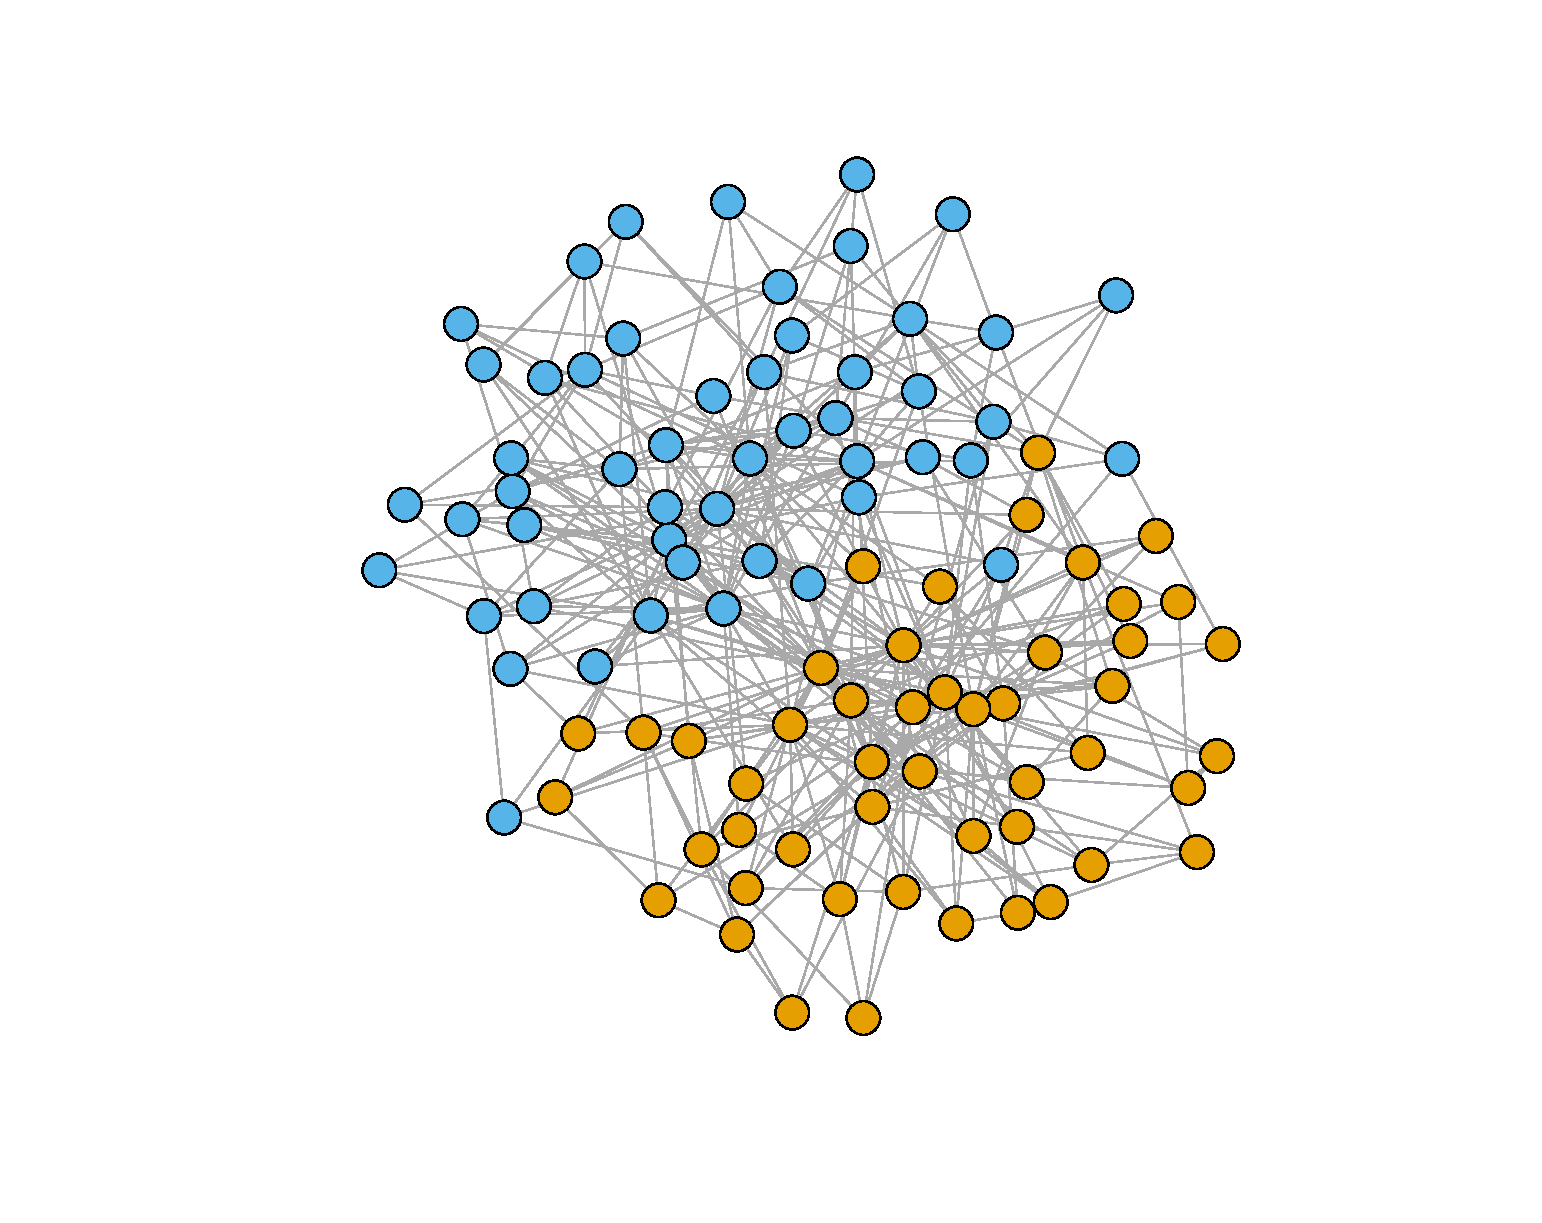
\includegraphics[width=\textwidth]{figs/barabasi_albert_example.pdf}
\caption{\label{fig:barabasi_albert_example} \small Example of the \texttt{barabasi\_albert\_communities} function with the community labels as vertex colors.}
\end{center}
\end{figure}


%\subsubsection{apply\_subgraphs}
Finally, it is worth mentioning the {\tt apply\_subgraphs()} function, which is used internally in the package, but has also been made available to the user because it can be very convenient. 
It simply calls a function \texttt{f} on each of the communities of a graph (treated as it's own \CRANpkg{igraph} object), acting as a wrapper for the \texttt{vapply} function. The communities are given as a membership vector \texttt{com}.
For a very simple example, we call it to obtain the order of each of the factions of the karate club graph:
\begin{example}
> apply_subgraphs(g=karate, com=V(karate)$Faction, f=gorder)
[1] 16 18
\end{example}


\section{An introductory example}
As a toy example we consider a famous benchmark social network: the Zachary's karate club graph~\citep{Zachary}.
First to showcase the graph randomization procedure {\tt rewireCpp}, we apply it to the Zachary's karate club graph with the default settings (positive weights with no upper bound, which suits this graph):
\begin{example}
> library(clustAnalytics)
> data(karate, package="igraphdata")
> rewired_karate <- rewireCpp(karate, weight_sel = "max_weight")
> par(mfrow=c(1,2), mai=c(0,0.1,0.3,0.1))
> plot(karate, main="karate")
> plot(rewired_karate, main="rewired_karate")
\end{example}
The resulting plots are shown in Figure \ref{fig:rewired_karate}.

\begin{figure}[htb!]  
\begin{center}
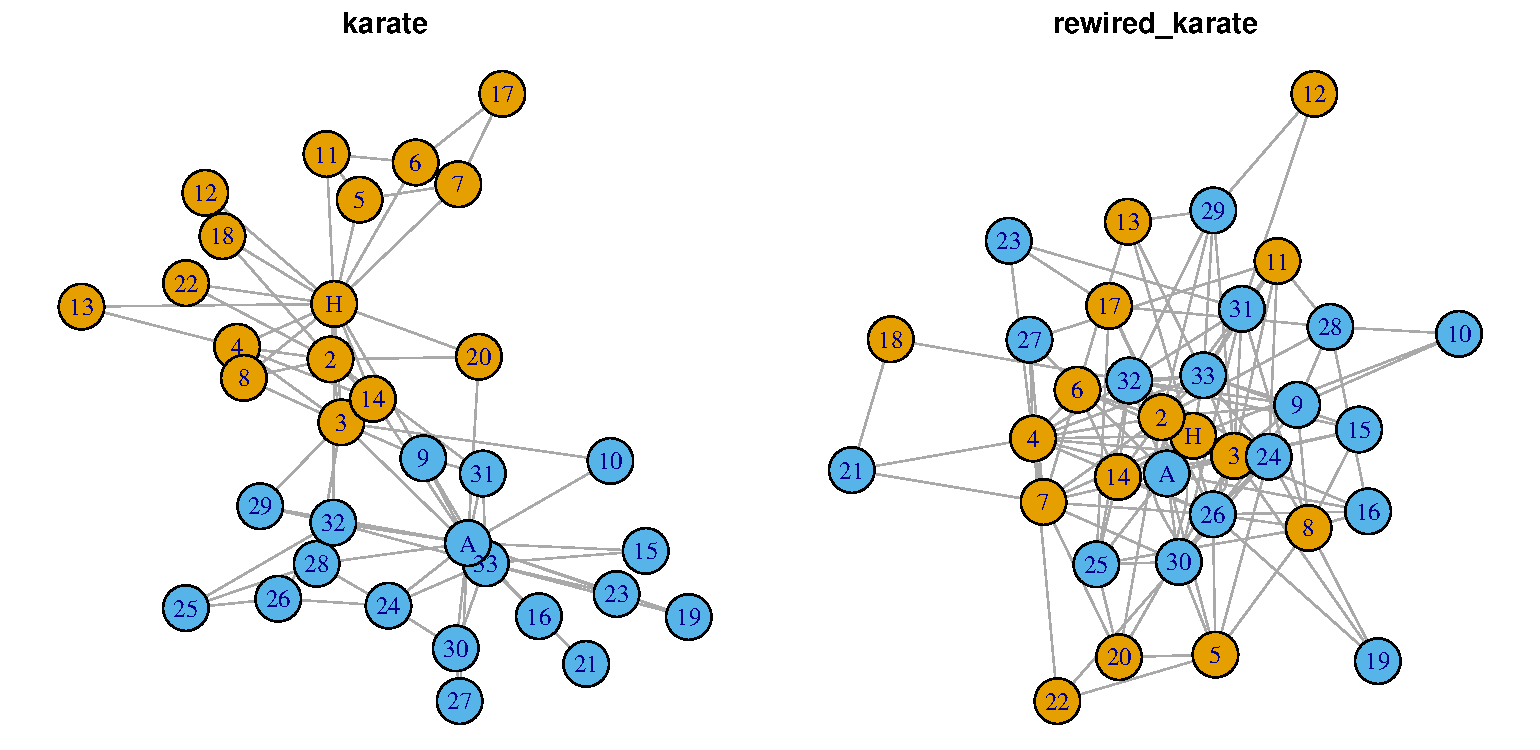
\includegraphics[width=\textwidth]{figs/karate_rewired_karate.pdf}
\caption{\label{fig:rewired_karate} \small Karate club graph before and after the edge randomization process. Colors represent the faction of each participant, the \textit{ground truth} clustering in this network.}
\end{center}
\end{figure}

The resulting rewired graph has lost its original communities centered around nodes $A$ and $H$, and if any alternative community structure appears, it is only due to chance. Now we continue with an analysis of significance and stability of some known clustering algorithms on  the Zachary's karate club graph. 

\subsection{Evaluating cluster significance} 
The function \texttt{evaluate\_significance} takes the graph and a list of clustering functions as arguments. If the graph has a known \textit{ground truth} community structure (such as the factions in the karate club), we can set \texttt{ground\_truth=TRUE} and set \texttt{gt\_clustering} as the membership vector to evaluate it and compare it to the results of the clustering algorithms. In our {\tt karate} graph the ground truth is available with {\tt V(karate)\$Faction}.
\begin{example}
> evaluate_significance(karate, ground_truth=TRUE,
+                       alg_list=list(Louvain=cluster_louvain, 
+                                     "label prop"= cluster_label_prop, 
+                                     walktrap=cluster_walktrap),
+                       gt_clustering=V(karate)$Faction)
                         Louvain  label prop    walktrap ground truth
size                  9.58823529 10.52941176 10.00000000  17.05882353
internal density      1.29491979  1.29766214  1.32254902   0.76885813
edges inside         50.35294118 59.17647059 51.82352941 104.82352941
av degree             5.05882353  5.29411765  5.05882353   6.14705882
FOMD                  0.26470588  0.29411765  0.26470588   0.41176471
expansion             3.47058824  3.00000000  3.47058824   1.29411765
cut ratio             0.14311885  0.12786548  0.14540629   0.07638889
conductance           0.25696234  0.22578022  0.25484480   0.09518717
norm cut              0.37937069  0.34206059  0.38131607   0.19090909
max ODF               0.43576990  0.42077566  0.51172969   0.38911607
average ODF           0.18336040  0.17884402  0.18493603   0.07498851
flake ODF             0.05882353  0.02941176  0.08823529   0.00000000
density ratio         0.87751142  0.88955342  0.86846364   0.90017702
modularity            0.41978961  0.41510519  0.41116042   0.37146614
graph_order          34.00000000 34.00000000 34.00000000  34.00000000
n_clusters            4.00000000  4.00000000  4.00000000   2.00000000
mean_cluster_size     8.50000000  8.50000000  8.50000000  17.00000000
coverage              0.74458874  0.77922078  0.74458874   0.90476190
global density ratio  0.75864388  0.76992481  0.74273256   0.80043860
VIdist_to_GT          0.90782167  0.82624391  0.87293838   0.00000000
\end{example}

If a \textit{ground truth} clustering has been provided, the row \texttt{VIdist\_to\_GT} indicates the variation of information distance \citep{varinformation} between that and each of the partitions. In this case the label propagation algorithm obtains the partition closest to the ground truth, while the Louvain algorithm is the furthest.

With the function \texttt{evaluate\_significance\_r} we compute the scoring functions as above, and we compare the results to those of a distribution of randomized graphs obtained with the rewiring method. %explained in Section \ref{switching_model}. 
The parameters of the rewiring method can be selected as 
shown in Table \ref{functions_table}, 
in this case we specify \texttt{weight\_sel="max\_weight"}, but we could also set an upper bound if appropriate to the graph. 
The resulting (default) table is shown below. 
This is a table with three columns per algorithm: the scores for the original graph, the
mean of the corresponding scores for the rewired graphs  and its percentile rank
within the distribution of scores for rewired graphs. 
If parameter {\tt table\_style = "string"}, the function instead returns a table with a column per algorithm where each element
is of the format "original|rewired(percentile)".


\begin{example}
> evaluate_significance_r(karate,
+                        alg_list=list(Lv=cluster_louvain,
+                                      "WT"= cluster_walktrap),
+                        weight_sel="max_weight", n_reps=100)
                              Lv          WT       Lv_r       WT_r Lv_perc WT_perc
size                  9.58823529 10.00000000  8.1670588  8.3705882    0.86    0.81
internal density      1.29491979  1.32254902  1.3911098  1.3728923    0.45    0.55
edges inside         50.35294118 51.82352941 29.1011765 39.1491176    0.99    0.82
av degree             5.05882353  5.05882353  3.6779412  3.8764706    1.00    0.98
FOMD                  0.26470588  0.26470588  0.1723529  0.1955882    0.98    0.87
expansion             3.47058824  3.47058824  6.2323529  5.8352941    0.00    0.02
cut ratio             0.14311885  0.14540629  0.2383912  0.2325316    0.00    0.00
conductance           0.25696234  0.25484480  0.4755745  0.4825704    0.00    0.01
norm cut              0.37937069  0.38131607  0.6760032  0.7073753    0.00    0.00
max ODF               0.43576990  0.51172969  0.6456208  0.6610584    0.00    0.03
average ODF           0.18336040  0.18493603  0.4450276  0.4626576    0.00    0.01
flake ODF             0.05882353  0.08823529  0.3423529  0.4088235    0.00    0.01
density ratio         0.87751142  0.86846364  0.7441942  0.7591046    1.00    1.00
modularity            0.41978961  0.41116042  0.1797852  0.1545682    1.00    1.00
clustering coef       0.54148426  0.61381521  0.4306771  0.4253075    0.76    0.87
graph_order          34.00000000 34.00000000 34.0000000 34.0000000    0.00    0.00
n_clusters            4.00000000  4.00000000  4.8200000  6.4800000    0.04    0.05
mean_cluster_size     8.50000000  8.50000000  7.2306667  5.7914928    0.72    0.85
coverage              0.74458874  0.74458874  0.5413420  0.5705628    1.00    0.98
global density ratio  0.75864388  0.74273256  0.5296269  0.5789977    1.00    0.98
\end{example}

%new addition
Depending on the application, more emphasis might be given to some of the metrics over others, but in most cases, those that take into account both internal and external connectivity (such as the modularity, conductance, or density ratio) will be the most relevant. Networks with significant clusters should result in values that are on the extremes of the distribution of rewired scores (so percentile rank one or close to one for the scores where higher values are better, and zero or close to zero for those where lower is better). The interpretation of the results is discussed in more detail in \citep{arratia2021clustering}.

If one simply wishes to compare clustering algorithms against each other, though, the distribution of rewired scores is not necessary and the \texttt{evaluate\_significance} function should be used instead.




\subsection{Applying scoring functions}
 
If it is the case that we already have some explicit community partition, but not the algorithm that produced it, we can assess its significance by applying the scoring functions directly to the network and the partition.
To apply all scoring functions at once use \texttt{scoring\_functions} with either {\tt type} local or global:

\begin{example}
> scoring_functions(karate, V(karate)$Faction, type="local")
  size internal density edges inside av degree      FOMD expansion  cut ratio
1   16        0.8250000           99  6.187500 0.5000000  1.375000 0.07638889
2   18        0.7189542          110  6.111111 0.3333333  1.222222 0.07638889
  conductance  norm cut   max ODF average ODF flake ODF density ratio modularity
1  0.10000000 0.1909091 0.3636364  0.05651941         0     0.9074074         NA
2  0.09090909 0.1909091 0.4117647  0.09140548         0     0.8937500         NA

> scoring_functions(karate, V(karate)$Faction, type="global")
         size internal density edges inside av degree      FOMD expansion  cut ratio
[1,] 17.05882        0.7688581     104.8235  6.147059 0.4117647  1.294118 0.07638889
     conductance  norm cut   max ODF average ODF flake ODF density ratio modularity
[1,]  0.09518717 0.1909091 0.3891161  0.07498851         0      0.900177  0.3714661
     graph_order n_clusters mean_cluster_size  coverage global density ratio
[1,]          34          2                17 0.9047619            0.8004386
\end{example}

Alternatively, we can apply the scoring functions individually. Each is called with the graph and the membership vector as arguments, and return a vector with the scores for each community:
\begin{example}
> cut_ratio(karate, V(karate)$Faction)
[1] 0.07638889 0.07638889

> conductance(karate, V(karate)$Faction)
[1] 0.10000000 0.09090909
\end{example}

 
A case in point are the clustering coefficient and transitivity.
As they can be applied to weighted graphs in general and not only to their partition into communities, they are simply called with the graph as the only argument:
\begin{example}
> weighted_clustering_coefficient(karate)
[1] 0.8127164
\end{example}

To be able to obtain the result for every community in the graph, we provide the function \texttt{apply\_subgraphs}; which given a graph, a membership vector and a scalar function that takes a graph as input, applies the function to every community and returns the vector of results. In this case it works as follows:
\begin{example}
> apply_subgraphs(karate, V(karate)$Faction, weighted_clustering_coefficient)
[1] 0.9514233 0.7783815
\end{example}







\subsection{Evaluating cluster stability}
Here we perform a nonparametric bootstrap to the karate club graph and the same selection of algorithms. For each instance, the set of vertices is resampled, the induced graph is obtained by taking the new set of vertices with the induced edges from the original graph, and the clustering algorithms are applied. Then, these results are compared to the induced original clusterings using the metrics mentioned above: the variation of information (VI), the normalized reduced mutual information (NRMI), and both adjusted and regular Rand index (Rand and adRand). Their exact definitions can be found in \citep{arratia2021clustering}.
\begin{example}
> boot_alg_list(g=karate, return_data=FALSE, R=99,
+               alg_list=list(Louvain=cluster_louvain, 
+                             "label prop"= cluster_label_prop, 
+                             walktrap=cluster_walktrap)) 
             Louvain label prop  walktrap
VI         0.2657555  0.3623330 0.2608622
NRMI       0.7024417  0.3415649 0.6959898
Rand       0.8584598  0.5969139 0.8609266
AdRand     0.6457648  0.2574423 0.6645099
n_clusters 5.9191919  5.1313131 6.3030303
\end{example}

Note that in this table the variation of information is a distance, so lower values indicate similar partitions, while for the NRMI, Rand, and adRand, higher values mean the partitions are more similar (1 means they are the same partition). 
% new addition 
Therefore, algorithms that produce stable clusters should result in low values of VI, and high values of the rest of metrics. In this example network we can see how the Louvain and walktrap algorithms have similar stability, while the label propagation algorithm performs much worse, and this is reflected in all metrics.



%%%%%%%%%%%%%%%%%%%%%%%%%%%%%%%%%%%%%%%%%%%%%%%%%%%%%%
\subsection{Clustering assessment on synthetic ground truth networks}
We can evaluate the significance and stability of clusters produced by a set of clustering algorithms on a  network with known community synthetically created with the stochastic block model (with function {\tt sample\_sbm}) or the preferential attachment model (with {\tt barabasi\_albert\_blocks}). The former produces a network with binomial degree distribution, and the latter  produces networks with scale-free degree distribution.

Let us  generate a graph from a stochastic block model in which we set very strong clusters: the elements in the diagonal of the matrix are much larger than the rest, so the probability of intra-cluster edges is much higher than that of inter-cluster edges.
\begin{example}
> pm <- matrix (c(.3, .001, .001, .003,
                .001, .2, .005, .002,
                .001, .005, .2, .001,
                .003, .002, .001, .3), nrow=4, ncol=4)
> g_sbm <- igraph::sample_sbm(100, pref.matrix=pm, block.sizes=c(25,25,25,25))
> E(g_sbm)$weight <- 1
> memb <- c(rep(1,25), rep(2,25), rep(3,25), rep(4,25))
> significance_table_sbm <- evaluate_significance(g_sbm, gt_clustering=memb)
> significance_table_sbm
                          Louvain   label prop     walktrap ground truth
size                  25.00000000 2.144000e+01  25.00000000  25.00000000
internal density       0.26500000 3.228846e-01   0.26500000   0.26500000
edges inside          79.50000000 6.968000e+01  79.50000000  79.50000000
av degree              3.18000000 3.010000e+00   3.18000000   3.18000000
FOMD                   0.43000000 4.000000e-01   0.43000000   0.43000000
expansion              0.24000000 5.800000e-01   0.24000000   0.24000000
cut ratio              0.00320000 6.907324e-03   0.00320000   0.00320000
conductance            0.03812704 1.091380e-01   0.03812704   0.03812704
norm cut               0.05064474 1.272639e-01   0.05064474   0.05064474
max ODF                0.29047619 3.554762e-01   0.29047619   0.29047619
average ODF            0.03789358 1.068777e-01   0.03789358   0.03789358
flake ODF              0.00000000 1.000000e-02   0.00000000   0.00000000
density ratio          0.98728802 9.778080e-01   0.98728802   0.98728802
modularity             0.69994949 6.663131e-01   0.69994949   0.69994949
clustering coef        0.28604270 3.302172e-01   0.28604270   0.28604270
graph_order          100.00000000 1.000000e+02 100.00000000 100.00000000
n_clusters             4.00000000 6.000000e+00   4.00000000   4.00000000
mean_cluster_size     25.00000000 1.666667e+01  25.00000000  25.00000000
coverage               0.96363636 9.121212e-01   0.96363636   0.96363636
global density ratio   0.97584906 9.498650e-01   0.97584906   0.97584906
VIdist_to_GT           0.00000000 3.403855e-01   0.00000000   0.00000000

\end{example}
%%%%%%%%%%%%%%%%%%%%%%%%%%%%%%%%%%%%%%%%%%%%%%%% 

 
In this case, \texttt{memb} is the membership vector of the ground truth clusters of the model. The clusters in the network are so strong that both the Louvain and walktrap algorithms manage to identify and match them exactly (their VI distance to the ground truth clustering is zero).

We now assess for stability of the clustering algorithms on this sbm graph:

\begin{example}
> b_sbm <- boot_alg_list(g=g_sbm, return_data=FALSE, R=99)
> b_sbm

             Louvain label prop  Walktrap
VI         0.1234341  0.1769217 0.1178832
NRMI       0.8536997  0.7841236 0.8656356
Rand       0.9411244  0.9230160 0.9472768
AdRand     0.8306925  0.7651778 0.8476909
n_clusters 6.9797980  7.7070707 7.4646465
\end{example}

We can clearly see that for all metrics, the results are much more stable than in the previous example, which makes sense because we purposefully created the SBM graph with very strong clusters.

\section{The \CRANpkg{clustAnalytics} package in context of related R packages}
The outstanding quality of \CRANpkg{clustAnalytics} is that it is a set of robust and efficient measures for assessing significance and stability  of clustering algorithms on graphs with the convenience of working with \CRANpkg{igraph} objects, which makes it a valuable complement to the  \CRANpkg{igraph} package \citep{igraph}. 
A revision of the {\em CRAN Task View: Cluster Analysis \& Finite Mixture Models} shows that there are very few packages devoted to assessing quality of clusters in general, and none for \CRANpkg{igraph}  graphs  as input. One could use in a limited manner some of the existing packages by converting \CRANpkg{igraph}  graphs to their adjacency matrices, but then quality evaluation follows different paradigms not quite pertaining to networks. 
For instance, the  package \CRANpkg{ClustAssess} \citep{clustassess} conceived for evaluating robustness of clustering of single-cell RNA sequences data 
using proportion of ambiguously clustered pairs, as well as similarity across methods and method stability using element-centric clustering comparison; \CRANpkg{sigclust} \citep{sigclust} which provides a single function to assess the statistical significance of splitting a data set into two clusters; \CRANpkg{clValid} \citep{clvalid} implements Dunn Index, Silhouette, Connectivity, Stability, BHI and BSI, for a statistical and biological-based validation of clustering results. None of these apply directly to \CRANpkg{igraph}  objects, and were not conceived for the analysis of clustering in social networks.
